\chapter{Iterative Closest Point (ICP)}
	\thispagestyle{empty}
	
	\newcommand{\ii}{\textbf{\emph{i}}}
	\newcommand{\jj}{\textbf{\emph{j}}}
	\newcommand{\kk}{\textbf{\emph{k}}}
	\newcommand{\qq}{\textbf{\emph{q}}}
	\newcommand{\pp}{\textbf{\emph{p}}}
	\newcommand{\vv}{\textbf{\emph{v}}}
	\newcommand{\xx}{\textbf{\emph{x}}}
	\newcommand{\uu}{\textbf{\emph{u}}}
	\newcommand{\ww}{\textbf{\emph{w}}}
	\newcommand{\aaa}{\textbf{\emph{a}}}
	\newcommand{\nn}{\textbf{\emph{n}}}
	\newcommand{\bb}{\textbf{\emph{b}}}
	
	\paragraph{}En esta sección explicaremos el primer algoritmo denominado \textit{Iterative Closest Point} (ICP), o Iteración del Punto más Cercano. Este algoritmo se utiliza en la etapa de alineación y su finalidad es que todas las tomas de datos estén referenciadas respecto al mismo sistemas de coordenadas. Este proceso también se suele denominar \textit{registro de datos} o \textit{data registration}. Veremos el método inicial propuesto en $ 1\,992 $ por Paul J.Besl and Neil D.MacKay \cite{ICPBesl}. Como veremos, este es un algoritmo complejo en tiempo y por ello, se tarda bastante en obtener los resultados deseados. Por ello, una vez estudiado el algoritmo se propondrán unas pequeñas mejoras del mismo que consistirán, básicamente, en el uso de las normales en cada punto para acelerar el proceso.\\
	
	Antes de explicar el algoritmo necesitamos unas nociones previas acerca de los \textit{cuaternios}. Los utilizaremos para la representación de las rotaciones en tres dimensiones, frente a la forma tradicional de representación matricial, y serán de gran ayuda a la hora de demostrar la convergencia del algoritmo. Tanto para la explicación de los cuaternios como su 
	uso en optimización se ha tomado como referencia \cite{QuatYan}.
\begin{figure}[h!]
	\begin{minipage}{0.5\textwidth}
		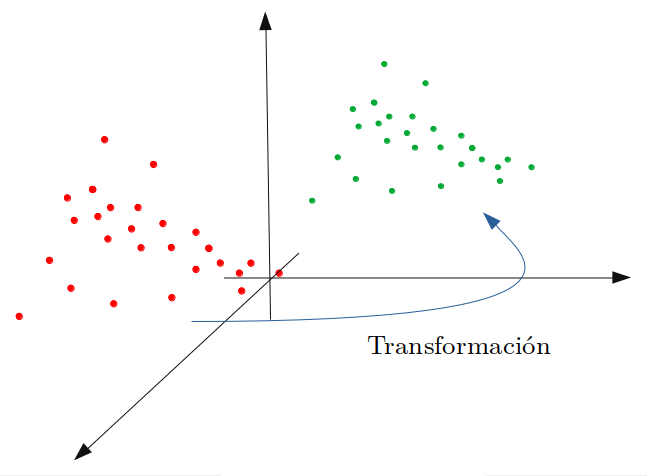
\includegraphics[width=0.8\linewidth, height=4.5cm]{Otros/Ej_Alineado_1} 
		%\caption*{Vista 1}
		%\label{fig:subim1}
	\end{minipage}
	\begin{minipage}{0.5\textwidth}
		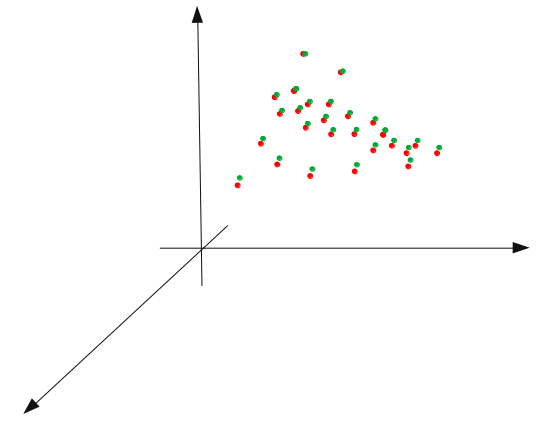
\includegraphics[width=0.8\linewidth, height=4.5cm]{Otros/Ej_Alineado_2}
		%\caption*{Vista 2}
		%\label{fig:subim2}
	\end{minipage}
	\caption{Antes y después de alinear dos nubes de puntos.}
\end{figure}

	\section{Cuaternios}
		Su desarrollo se atribuye a W.R Hamilton en $ 1\,843 $.  Son una extensión de los números complejos. Mientras que estos últimos solo incluyen la unidad imaginaria $ \ii$, los cuaternios añaden la unidades imaginarias $ \ii, \jj, \kk $ tales que:
		\begin{equation*}
			\ii^2 = \jj^2 = \kk^2 = \ii\jj\kk = -1.
		\end{equation*} 
		
		Así, el conjunto de los cuaternios se define como:
		\begin{equation*} 
			\lbrace q_0 + q_1 \ii + q_2 \jj + q_3 \kk : q_0, q_1, q_2, q_3 \in \RR \rbrace.
		\end{equation*}
		Podemos ver a los cuaternios como la suma de un escalar $ q_0 \in \RR$ y de un vector de $ \RR^3 $ que llamamos $ \qq = (q_1,q_2,q_3)$ donde la base usual de $ \RR^3 $ viene dada por los vectores unitarios $ \ii =(1,0,0), \jj = (0,1,0) \text{ y } \kk = (0,0,1)$. Notaremos $
		q = q_0 + \qq =  q_0 + q_1 \ii + q_2 \jj + q_3 \kk $. Si la parte escalar es 0, es decir, $ q_0 = 0 $ hablamos de un \textit{cuaternio puro}. Por otro lado, a modo de notación podemos expresar $ q $ como vectores de cuatro dimensiones, es decir, si $ q $ es de la forma mencionada podemos pensar que $ q = (q_0, q_1, q_2, q_3) \in \RR^4 $.
		
		\begin{subsection}{Suma y producto}
			La suma de dos cuaternios se realiza componente a componente. Por ello, dados los cuaternios
		 	\begin{equation*}
		 	\begin{split}
		 	q &= q_0 + q_1 \ii + q_2 \jj + q_3 \kk = q_0 + \qq \\
		 	p &= p_0 + p_1 \ii + p_2 \jj + p_3 \kk = p_0 + \pp,
		 	\end{split}
		 	\end{equation*}
			definimos su suma de la siguiente manera:
			
			\begin{equation*}
			q + p= (q_0 + p_0 )+ (q_1 + p_1 )\ii + (q_2 + p_2 ) \jj + (q_3 + p_3 ) \kk.
			\end{equation*}
			Es directo comprobar que la suma es asociativa y conmutativa.\\
			
			El producto, por su parte, sigue una serie de reglas introducidas por Hamilton y que las presentamos a continuación:
			\begin{equation*}
			\begin{split}
			\ii^2 &= \jj^2 = \kk^2 = \ii\jj\kk = -1.\\
			\ii\jj &= 	\kk = 	-\jj\ii.\\
			\jj\kk &= \ii = -\kk\jj. \\
			\kk\ii &= 	\jj = -	\ii\kk.
			\end{split}
			\end{equation*}
			Por ello, el producto de dos cuaternios viene dado por:
			\begin{equation*}
			\begin{split}
			pq&= (p_0 + p_1 \ii + p_2 \jj + p_3 \kk)(q_0 + q_1 \ii + q_2 \jj + q_3 \kk) \\
			&= p_0q_0 - (p_1q_1+p_2q_2+p_3q_3) + p_0(q_1\ii+q_2\jj+q_3\kk) \\
			&+ q_0(p_1\ii+p_2\jj+p_3\kk) + (p_2q_3-p_3q_2)\ii +  (p_3q_1-p_1q_3)\jj \\
			&+ (p_1q_2-p_2q_1)\kk.
			\end{split}
			\end{equation*}
			Podemos simplificar esta expresión usando el producto escalar y vectorial de $ \RR^3 $ quedando la expresión más concisa:
			\[
			pq = p_0q_0 - \langle \pp , \qq \rangle + p_0\qq + q_0\pp + \pp \times \qq.
			\]			
			No es difícil comprobar que el producto es asociativo y distributivo respecto a la suma pero no conmutativo. La no conmutatividad se puede observar del hecho de que el producto vectorial no es conmutativo. Es importante notar que los cuaternios son cerrados bajo la suma y el producto definidos anteriormente. En el caso del producto, obtenemos otro cuaternio con parte escalar $ p_0q_0 -  \langle \pp , \qq \rangle $ y vector $ p_0\qq + q_0\pp + \pp \times \qq $. \\
			
			Este conjunto con las operaciones de suma y producto forman un anillo no conmmutativo. El elemento neutro para la suma sería un cuaternio donde $ q_0 = q_1 = q_1 = q_3 = 0 $ y dado un elemento $  q = q_0 + \qq $ su opuesto sería $ -q = -q_0-\qq  $. Por su parte, el elemento neutro para el producto sería un cuaternio con parte real $ 1 $ y vector $ \mathbf{0} $.
		\end{subsection}
	
		\subsection{Conjugado, norma e inverso}
			Sea el cuaternio dado por $ q = q_0 + q_1 \ii + q_2 \jj + q_3 \kk $. Notamos a su \textit{conjugado} como $ q^* $ y que se define como:
			\[
			q^* = q_0 - \qq = q_0 - q_1 \ii - q_2 \jj - q_3 \kk.
			\]
			
			De la definición obtenemos las siguientes propiedades básicas del manejo de cuaternios:
			\begin{equation*}
			\begin{split}
			(q^*)^* &= q - (-\qq) = q.\\
			q + q^* &= q_0.\\
			 q q^*= q^*q & = (q_0+\qq)(q_0+\qq) \\
			&= q_0q_0 - \langle-\qq, \qq \rangle + q_0\qq + (-\qq)q_0 + (-\qq) \times \qq \\
			&= q_0^2 + \langle\qq , \qq \rangle\\
			&= q_0^2 + q_1^2 + q_3^2 + q_4^2 \\
			& = q_0^2 + \norm{\qq}.
			\end{split}
			\end{equation*}
			En la última expresión $ \norm{\cdot} $ representa la norma usual de $ \RR^3 $. Podemos probar que dados dos cuaternio $ p,q $ se cumple que $ (pq)^* = q^*p^* $. Efectivamente:
			\begin{equation*}
			\begin{split}
			(pq)^* &= p_0q_0 - \langle \pp , \qq \rangle - p_0\qq - q_0\pp - \pp \times \qq \\
			 &= p_0q_0 - \langle \pp , \qq \rangle - p_0\qq - q_0\pp + \qq \times \pp \\
			 &= q_0p_0 - \langle -\qq , -\pp \rangle + q_0(-\pp)+p_0(-\qq) + (-\qq) \times (-\pp)\\
			 &= (q_0-\qq)(p_0-\pp)\\
			 &= q^* p^*.
			\end{split}
			\end{equation*}
			
			La \textit{norma} de un cuaternio se nota como $ \abs{q} $ y se define como $ \abs{q} = \sqrt{q^*q}$. Usando la propiedad anterior de que el conjugando del producto es el producto de los conjugados cambiados de orden llegamos a:
			\begin{equation*}
			\begin{split}
			\abs{pq}^2 &= (pq)^*(pq) \\
			&= q^*p^*pq \\
			&=  q^*\abs{p}^2 q \\
			&= \abs{p}^2q^*q \\
			&= \abs{p}^2\abs{q}^2.
			\end{split}
			\end{equation*}
			
			Por su parte, el \textit{inverso} de un cuaternio se define como:
			\[
			q^{-1} = \frac{q^*}{\abs{q}^2}.
			\]
			Se cumple que: 
			\[
			qq^{-1} =q^{-1}q =  \frac{q^*}{\abs{q}^2} q = \frac{\abs{q}^2}{\abs{q}^2} = 1.
			\]
			En el caso de que $ q $ sea unitario (tenga norma uno) tenemos que $ q^{-1} = q^* $. Notar que los cuaternios unitarios forman un grupo con operación interna el producto. 
			
	
		\subsection{Cuaternios y rotaciones}\label{Cuat+Rot}
		El grupo de rotaciones en $ \RR^3 $ alrededor de un eje que pasa por el origen, y que lo notamos como $ SO(3) $, está formado por las matrices reales 3x3 que son ortogonales (su inversa coincide con la traspuesta) y tienen determinante igual a 1. \\
		
		Nos surge entonces la siguiente pregunta: ¿por qué usar los cuaternios para representar dichas rotaciones? En primer lugar, el uso de matrices resulta redundante. Las rotaciones en $ \RR^3 $ tienen básicamente tres grados de libertad: dos para la representación del eje (dado en coordenadas esféricas, por ejemplo) y uno para el ángulo de giro. Por ello, al usar matrices estamos usando demasiados elementos. Con el uso de los cuaternios seguimos teniendo redundancia pero solo por un valor más. Además, a partir de un eje de rotación y un ángulo de giro se puede construir fácilmente el cuaternio asociado, y del mismo modo, obtener el eje y ángulo a partir del cuaternio, mientras que en matrices dicha relación no es tan clara.  También reducimos el número de operaciones necesarias a la hora de componer dos rotaciones. En la multiplicación de matrices se necesitan 27 multiplicaciones y 18 sumas y en el producto de cuaternios (veremos que esta es la operación de composición) 16 multiplicaciones y 20 sumas. Por otro lado, podemos usar los \textit{ángulos de Euler} para identificar las rotaciones que utiliza el número de valores mínimo. Sin embargo, con este sistema podemos llegar a una situación no deseada que se conoce como \textit{gimbal lock} o \textit{bloqueo del cardán} \cite{QuatPowerPoint}.  Este fenómeno se produce cuando los tres ejes están en el mismo plano y nos produce la pérdida de uno de los ejes de giro. Por estas razones, entre otras, los cuaternios se conocen generalmente como la ``mejor'' manera para representar las rotaciones en el espacio. Más específicamente, la representación de las rotaciones en tres dimensiones se hace mediante cuaternios unitarios. Veamos el proceso: \\
		
		Sea $ q $ un cuaternio unitario de la forma $ q = q_0 + \qq $. Al tener norma uno tenemos que $ \abs{q}^2 = q_0^2 + \norm{\qq}^2 = 1 $. Así, como $ (q_0, \norm{\qq}) \in \mathbb{S}^1 $, existe un único ángulo $ \theta \in \lbrack 0,2\pi ) $ que cumple: 	
		\begin{equation*}
			\begin{cases}
			 \cos^2 \theta = q_0^2 \\
			 \sen^2\theta = \norm{\qq}^2 ,
			\end{cases}
		\end{equation*}
		y podemos escribir ahora $ q $ en términos de $ \theta \text{ y } \uu$ con $ \uu = \mathbf{\qq}/\norm{\qq}$ de la siguiente manera: $ q = \cos\theta + \uu\sen\theta $. \\
		
		Dado el cuaternio unitario $ q $, definimos la aplicación $ L_q $ dada por:
		\begin{equation*}
			\begin{split}
			L_q:\RR^3 &\longrightarrow \RR^3 \\
			\vv &\longmapsto L_q(\vv) = q\vv q^* =(q_0^2-\norm{\qq}^2)\vv + 2\langle\qq , \vv\rangle \qq + 2q_0(\qq \times \vv)
			\end{split}
		\end{equation*} 
		La aplicación $ L_q $ está bien definida y no tenemos problema en multiplicar un vector por un cuaternio, ya que podemos ver un vector como un cuaternio puro. Hacemos ahora dos observaciones interesantes que nos hacen pensar, en principio, que la aplicación $ L_q $ actúa como una rotación con eje $ \qq $.
	
		\bigskip
		\begin{observacion}
			La aplicación $ L_q $ no cambia la norma de $ \vv \in \RR^3 $.
		\end{observacion}
		En efecto:	
		\begin{equation*}
			\norm{L_q(\vv)} = \norm{q\vv q^*} = \abs{q} \norm{\vv} \abs{q^*} = \norm{\vv}.
		\end{equation*}
		
		\begin{observacion}\label{NoCambiaEje}
			Si $ \vv = k\qq $ con $ k \in \RR $ entonces la dirección de $ \vv $ no cambia al aplicarle $ L_q $.
		\end{observacion}	
		Usando la definición de $ L_q $ y al ser $ q $ unitario llegamos a:
		\begin{equation*}
		\begin{split}
		L_q(\vv) &= q \vv q^* \\
		&= (q_0^2-\norm{\qq}^2)(k\qq) + 2\langle\qq, k\qq\rangle\qq + 2q_0(\qq \times k\qq) \\
		&= k(q_0^2-\norm{\qq}^2)\qq + 2k\langle\qq, \qq\rangle\qq + 2kq_0(\qq \times \qq) \\
		&= k(q_0^2-\norm{\qq}^2)\qq + 2k\norm{\qq}^2\qq \\
		&= k(q_0^2+\norm{\qq}^2)\qq \\
		&= k\qq.
		\end{split}
		\end{equation*}
		\bigskip
		
		Antes de formalizar la ``intuición'' que nos han dado las observaciones anteriores necesitamos otra que es un poco más técnica. 
	
		\bigskip
		\begin{observacion}
			La aplicación $ L_q $ es lineal, es decir, dados $ a_1,a_2 \in \RR \text{ y } \vv_1, \vv_2 \in \RR^3$ se tiene que $ L_q(a_1\vv_1 + a_2 \vv_2) = a_1 L_q (\vv_1) + a_2 L_q(\vv_2) $.
		\end{observacion}
		Se obtiene por la distributividad del producto:
		\begin{equation*}
		\begin{split}
		L_q(a_1\vv_1 + a_2 \vv_2 ) &=q(a_1\vv_1 + a_2 \vv_2)q^* \\
		&=q(a_1\vv_1 q^* + a_2 \vv_2 q^*) \\
		&=qa_1\vv_1 q^*  + qa_2 \vv_2 q^*\\
		&= a_1q\vv_1 q^*  + a_2 q\vv_2 q^* \\
		&=a_1 L_q (\vv_1) + a_2 L_q(\vv_2).
		\end{split}			
		\end{equation*}
		\bigskip
		
		El teorema que exponemos a continuación es clave y nos indica que dado un vector y ángulo podemos construir un cuaternio $ q $ tal que $ L_q $ representa la rotación deseada.
		
		\begin{teoremaBox}
			Para cualquier cuaternio $ q = q_0 + \qq = \cos \theta/2 + \uu \sen \theta/2$ y para cualquier vector $ \vv \in \RR^3 $ tenemos que $ L_q(\vv) $ es equivalente a la rotación con eje de giro $ \uu $ y ángulo $ \theta $. 
		\end{teoremaBox}
	
\begin{proof}
Tomamos $ \vv \in \RR^3 $ y lo expresamos en términos de $ \qq $ y $ \lbrace\qq \rbrace^\perp $. De este modo, $ \vv = \aaa + \nn $ donde $ \aaa $ es la componente respectiva a $ \qq $ y $ \nn $ la de $ \lbrace\qq \rbrace^\perp $. Bajo $ L_q $, $ \aaa $ se queda invariante por la observación \ref{NoCambiaEje} mientras que $ \nn $ rota un ángulo $ \theta $ alrededor de $ \qq $. En efecto:
\begin{equation*}
	\begin{split}
	L_q(\nn) &= (q_0^2-\norm{\qq}^2)\nn + 2\langle\qq , \nn\rangle\qq + 2q_0(\qq \times \nn)\\
		&= (q_0^2-\norm{\qq}^2)\nn + 2q_0(\qq \times \nn) \\
		&= (q_0^2-\norm{\qq}^2)\nn + 2q_0\norm{\qq}(\uu \times \nn),
			\end{split}
			\end{equation*} 	
			donde la última igualdad se debe a que $ \uu = \qq / \norm{\qq} $. Notamos $ \nn_0= \uu \times \nn$. Es claro por ello que $ \nn_0 $ es perpendicular tanto a $ \uu $ (y por ello también a $ \qq $) y a $ \nn $. Obtenemos: 
			\begin{equation}\label{fmla}
				L_q(\nn) =  (q_0^2-\norm{\qq}^2)\nn + 2q_0\norm{\qq}\nn_0.
			\end{equation} 
			Tanto $ \nn_0 \text{ como }  \nn $ tienen la misma longitud:
			\begin{equation*}
				\norm{\nn_0} = \norm{\nn \times \uu} = \norm{\uu \times \nn} = \norm{\nn}\norm{\uu}\sen(\pi/2) = \norm{\nn}.
			\end{equation*}
			Escribimos \ref{fmla} es términos de $ \theta $:
			\begin{equation*}
			\begin{split}
			L_q(\nn) &= (\cos^2\frac{\theta}{2} - \sen^2\frac{\theta}{2})\nn + (2\cos^2\frac{\theta}{2}\sen^2\frac{\theta}{2})\nn_0 \\
			&= \cos\theta\nn + \sen\theta\nn_0.
			\end{split}
			\end{equation*}
			Las últimas igualdades se han obtenido mediante las fórmulas del seno y coseno del ángulo doble. Vemos que el vector resultante es la rotación de $ \nn $ un ángulo $ \theta $ en el plano definido por $ \nn \text{ y } \nn_0 $. Claramente el vector resultante es perpendicular al eje de rotación ya que $ \nn$ y $ \nn_0 $ pertenecen a $ \lbrace \qq \rbrace ^\perp$. La demostración termina usando la linealidad que nos aporta la observación 3.
		\end{proof}
	 	\bigskip
	 	
En resumen, dados $ \qq \in \RR^3$ y $ \theta \in \RR$ representamos la rotación de ángulo de giro $ \theta $ alrededor del eje $ \qq$ por $  q = \cos\frac{\theta}{2} + \frac{\qq}{\norm{\qq}} \sen \frac{\theta}{2} $ y la aplicamos a un vector $ \uu \in \RR^3 $ mediante $ L_{q} (\uu) = q\uu q^* $.  \\
		
		Finalmente, exponemos la siguiente observación que nos indica la relación de la composición de rotaciones con su representación mediante cuaternios.
		\bigskip
		\begin{observacion}
			 Sean p,q dos cuaternios unitarios, entonces $ L_q \circ L_p = L_{qp} $. 
		\end{observacion}
		Como $ p \text{ y } q$ son unitarios entonces $ pq $ también lo es. Notamos $ L_p(\uu) = \vv \text{ y } L_q(\vv) = (L_q \circ L_p)(\uu) = \ww $. Obtenemos:
		\begin{equation*}
		\begin{split}
			\ww &= L_q(\vv) = q\vv q^* \\
			&= q(p\uu p^*) q^*\\ 
			&= (qp)\uu(qp)^* \\ 
			&= L_{qp}(\uu).
		\end{split}
		\end{equation*} 
		\bigskip
		
		De este modo, hemos obtenido que la composición de rotaciones representadas en cuaternios se obtiene mediante la multiplicación de los cuaternios que representa cada una de las rotaciones por separado. \\
				
	
	\section{Cuaternios y optimización}\label{optimizacion}
Sea $ P = \{\pp_i\} $ un conjunto con $ N_p $ puntos que queremos alinear tomando como sistema de referencia otro conjunto $ X = \{\xx_i\} $ de tamaño $ N_x $. Suponemos que $ N_p = N_x $ y que cada $ \pp_i \in P $ corresponde con $ \xx_j \in X $ siempre y cuando $ i = j $. Esta correspondencia hace referencia a que conocemos cómo se relacionan los puntos de ambos conjuntos y por ello $ p_i $ es el punto $ x_i $ pero en un sistema de referencia diferente. Aclararemos esta relación en apartados siguientes. Suponer que ambos conjuntos de puntos tienen el mismo tamaño puede parecer bastante restrictivo en un primer momento pero posteriormente veremos que no es el caso. De este modo, el problema consiste en encontrar una rotación $ R $ y una traslación $ \bb $ que nos proporcionen las distancias más pequeñas entre los puntos. Así, la función objetivo a ser minimizada es:
		
		\begin{equation}\label{min}
		F (R,\bb) = \sum_{i = 1}^{N_p} \norm{R\pp_i + \bb - \xx_i}^2.
		\end{equation}
		En primer lugar, obtenemos los centroides de ambos conjuntos de puntos. Recordando que que $ N_p = N_x $, los notamos como:
		\[
		\bar{\pp} = \frac{1}{N_p} \sum_{i=i}^{N_p} \pp_i,  \quad \bar{\xx} = \frac{1}{N_p} \sum_{i=i}^{N_p} \xx_i.
		\]
		A continuación, obtenemos las coordenadas relativas a los centroides:
		\[
		\pp_i' = \pp_i - \bar{\pp}, \quad \xx_i' = \xx_i - \bar{\xx}.
		\]
		Notamos que se cumple que:
		\begin{equation}\label{cen0}
		\begin{split}
			\sum_{i=1}^{N_p} \pp_i' = \sum_{i=1}^{N_p} (\pp_i - \bar{\pp}) = \sum_{i=1}^{N_p} \pp_i - N_p\bar{\pp} = \sum_{i=1}^{N_p} \pp_i - N_p\frac{1}{N_p} \sum_{i=i}^{N_p} \pp_i = 0, \\
			\sum_{i=1}^{N_p} \xx_i' = \sum_{i=1}^{N_p} (\xx_i - \bar{\xx}) = \sum_{i=1}^{N_p} \xx_i - N_p\bar{\xx} = \sum_{i=1}^{N_p} \xx_i - N_p\frac{1}{N_p} \sum_{i=i}^{N_p} \xx _i = 0. 
		\end{split}
		\end{equation}		
		Expresando ahora \eqref{min} en términos de $ \pp_i, \xx_i, \bar{\pp} \text{ y } \bar{\xx}$:
		\begin{equation*}
		\begin{split}
		\sum_{i = 1}^{N_p} \norm{R\pp_i + \bb - \xx_i}^2 &= \sum_{i = 1}^{N_p} \norm{R(\pp_i' + \bar{\pp} ) + \bb - (\xx_i' + \bar{\xx})}^2 \\
		&=\sum_{i = 1}^{N_p} \norm{R\pp_i' -\xx_i' + R\bar{\pp}  + \bb - \bar{\xx}}^2 \\
		&= \sum_{i = 1}^{N_p} \langle R\pp_i' -\xx_i' + R\bar{\pp}  + \bb - \bar{\xx}, R\pp_i' -\xx_i' + R\bar{\pp}  + \bb - \bar{\xx} \rangle.
		\end{split}
		\end{equation*} 
		Para simplificar la escritura, llamamos $ a_i = R\pp_i' -\xx_i' \text{ y } c = R\bar{\pp}  + \bb - \bar{\xx}$. Como el producto escalar es bilineal obtenemos: 
		\begin{equation*}
		\begin{split}
		\sum_{i = 1}^{N_p} \langle a_i + c, a_i + c\rangle &= \sum_{i = 1}^{N_p} \langle a_i + c, a_i \rangle + \sum_{i = 1}^{N_p} \langle a_i + c, c\rangle\\ 
		& = \sum_{i = 1}^{N_p} \langle a_i, a_i \rangle + \sum_{i = 1}^{N_p} \langle c, a_i\rangle + \sum_{i = 1}^{N_p} \langle a_i, c \rangle + \sum_{i = 1}^{N_p} \langle c, c\rangle \\
		& = \sum_{i = 1}^{N_p} \norm{a_i}^2 + 2\sum_{i = 1}^{N_p} \langle a_i, c\rangle + \sum_{i = 1}^{N_p} \norm{c}^2 \\
		& = \sum_{i = 1}^{N_p} \norm{a_i}^2 + 2\sum_{i = 1}^{N_p} \langle a_i, c\rangle + N_p \norm{c}^2 \\
		& = \sum_{i = 1}^{N_p} \norm{a_i}^2 + 2 \langle \sum_{i = 1}^{N_p} a_i, c\rangle + N_p \norm{c}^2.
		\end{split}
		\end{equation*} 
		Si sustituimos $ a_i $ por su valor en el término central y usamos \eqref{cen0}:
		\begin{equation*}
			\sum_{i = 1}^{N_p} a_i = \sum_{i = 1}^{N_p} (R\pp_i' -\xx_i') = \sum_{i = 1}^{N_p} R\pp_i' - \sum_{i = 1}^{N_p}\xx_i' = 0.
		\end{equation*} 
		Por lo tanto: 
		\begin{equation*}
		\begin{split}
		\sum_{i = 1}^{N_p} \norm{R\pp_i + \bb - \xx_i}^2 &= \sum_{i = 1}^{N_p} \norm{R\pp_i' -\xx_i'}^2 + N_p\norm{R\bar{\pp}  + \bb - \bar{\xx}}^2.
		\end{split}
		\end{equation*} 
		La traslación $ \bb $ buscada debería hacer 0 el segundo término obteniendo entonces:
		\[\bb = R\bar{\pp}  + \bar{\xx}.
		\]
		Ahora, para obtener la mejor rotación utilizamos el primero término. Reescribiendo la misma llegamos a:
		\begin{equation*}
		\begin{split}
		\sum_{i = 1}^{N_p} \norm{R\pp_i' -\xx_i'}^2 &= \sum_{i = 1}^{N_p} \langle R\pp_i' -\xx_i', R\pp_i' -\xx_i' \rangle \\
		&= \sum_{i=1}^{N_p} \langle R \pp_i' , R \pp_i' \rangle - 2\sum_{i=1}^{N_p}\langle R\pp_i', \xx_i'\rangle + \sum_{i=1}^{N_p} \langle \xx_i', \xx_i'\rangle \\
		&= \sum_{i=1}^{N_p} RR^T \norm{\pp_i'}^2 - 2\sum_{i=1}^{N_p}\langle R\pp_i', \xx_i'\rangle + \sum_{i=1}^{N_p} \norm{\xx_i'}^2\\
		&= \sum_{i=1}^{N_p} (\norm{\pp_i'}^2 + \norm{\xx_i'}^2)- 2\sum_{i=1}^{N_p}\langle R\pp_i', \xx_i'\rangle.
		\end{split}
		\end{equation*}
		El primer término no depende de la rotación por lo que no influirá en el cálculo. Y el segundo, que sí depende de $ R $, hará que  $ \sum_{i = 1}^{N_p} \norm{R\pp_i' -\xx_i'}^2 $ sea mínimo cuando tome su valor máximo al estar restando. Nos encontramos ahora en un problema de maximización. Usamos ahora la representación en cuaternios de las rotaciones y que hemos introducido en la sección \ref{Cuat+Rot}. Sea $ q  $ el cuaternio (unitario) que representa la misma rotación que la matriz $ R $. Tenemos que maximizar:
		
		\begin{equation*}
		\sum_{i=1}^{N_p}\langle q\pp_i'q^*, \xx_i'\rangle.
		\end{equation*}
		Aplicando la definición del producto de cuaternios no es difícil probar que: 
		%%% (¡¡ REVISAR PROCEDIMIENTO !!):
		
		\begin{equation}\label{1.4}
		\sum_{i=1}^{N_p}\langle q\pp_i'q^*, \xx_i'\rangle = 	\sum_{i=1}^{N_p}\langle q\pp_i', \xx_i'q\rangle.
		\end{equation}
		Visto $ q $ como un vector de $ \RR^4 $ tenemos que $ q = (q_0, q_1, q_2, q_3)^T$. También vemos los puntos $ \pp_i' $ y $ \xx_i' $ como cuaternios puros notando a sus componentes como $ \pp_i' = (0, p_{i1}', p_{i2}', p_{i3}' ) $ y $ \xx_i' = (0, x_{i1}', x_{i2}', x_{i3}' ) $ para $ i=1,...,N_p $.\\
		
		Nuestro propósito ahora es escribir los sumandos de \eqref{1.4} como producto matricial. Construimos las matrices para cada $ i= 1, \dots, N_p$: 
		%%% (¡¡ VER CÓMO SE CONSTRUYEN!!):
		
		\begin{equation}\label{covDife}
		P_i = \begin{pmatrix}
		0 & -p_{i1}' &-p_{i2}' &-p_{i3}' \\
		p_{i1}' & 0 & p_{i3}'& -p_{i2}' \\
		p_{i2}' & -p_{i3}' & 0 & p_{i1}' \\
		p_{i3}' & p_{i2}' & -p_{i1}' & 0\\
		\end{pmatrix}
		\text{, }
		X_i = \begin{pmatrix}
		0 & -x_{i1}' &-x_{i2}' &-x_{i3}' \\
		x_{i1}' & 0 & -x_{i3}'& x_{i2}' \\
		x_{i2}' & x_{i3}' & 0 & -x_{i1}' \\
		x_{i3}' & -x_{i2}' & x_{i1}' & 0\\
		\end{pmatrix}.
		\end{equation}	
		Observamos que $ q\pp_i' $ coincide con $ P_i q$  y que $ \xx_i'q $ hace lo mismo con $ X_i q $, sustituimos en \eqref{1.4}:
		\begin{equation*}
		\begin{split}
		\sum_{i=1}^{N_p}\langle q\pp_i', \xx_i'q\rangle &=  \sum_{i=1}^{N_p}\langle P_i q,  X_ix\rangle\\
		&= \sum_{i=1}^{N_p} \langle q ,P_i^T X_i q \rangle\\
		&= \langle q , \left( \sum_{i=1}^{N_p}P_i^T X_i\right) q \rangle.
		\end{split}
		\end{equation*}
		Podemos comprobar sin dificultad que la matriz $ P_i^T X_i $ es simétrica por lo que la suma de ellas también lo es. Llameamos a su suma
		\begin{equation}\label{MSum}
			M = \sum_{i = 1}^{N_p}P_i^TX_i.
		\end{equation}
 Como $ M $ es simétrica podemos asegurar que todos sus valores propios son reales. Sean $ \lambda_1 \geq \lambda_2 \geq \lambda_3 \geq \lambda_4 $ dichos valores propios (tenemos en cuentas las multiplicidades) y $ \vv_1, \vv_2, \vv_3, \vv_4 $ sus correspondientes vectores propios unitarios asociados. Sabemos que vectores propios asociados a diferentes valores propios son perpendiculares entre sí. Si corresponden al mismo podemos elegirlos de tal manera para que también sean ortogonales.  Por lo tanto, podemos escribir el cuaternio $ q $ como combinación lineal de vectores propios:
		\[
		q = \alpha_1 \vv_1 + \alpha_2 \vv_2 + \alpha_3 \vv_3 + \alpha_4 \vv_4,
		\]
		tenemos entonces que la matriz $ M $ expresada en la base $ \{ \vv_1, \vv_2, \vv_3, \vv_4\} $ de sus vectores propios es diagonal  con $ M = diag(\lambda_1, \lambda_2, \lambda_3, \lambda_4) $. Así:
		\begin{equation*}
		\begin{split}
		\langle q , M q \rangle &= \langle \alpha_1 \vv_1 + \alpha_2 \vv_2 + \alpha_3 \vv_3 + \alpha_4 \vv_4, M(\alpha_1 \vv_1 + \alpha_2 \vv_2 + \alpha_3 \vv_3 + \alpha_4 \vv_4 )\rangle \\
		&=  \langle \alpha_1 \vv_1 + \alpha_2 \vv_2 + \alpha_3 \vv_3 + \alpha_4 \vv_4, \lambda_1\alpha_1 \vv_1 + \lambda_2\alpha_2 \vv_2 + \lambda_3\alpha_3 \vv_3 + \lambda_4\alpha_4 \vv_4 \rangle \\
		&=  \lambda_1\alpha_1^2 + \lambda_2\alpha_2^2 + \lambda_3\alpha_3^2 + \lambda_4\alpha_4^2.
		\end{split}
		\end{equation*}
		De este modo, 
		%%%(USAR LEMA 2.1 MATEMÁTICAS ??) 
		$ \langle q , M q \rangle $ es máximo cuando $ \alpha_1^2 = 1 $ y $ \alpha_2^2 = \alpha_3^2 = \alpha_4^2 = 0 $ ya que al ser $ q $ unitario debe cumplir $ \alpha_1^2 + \alpha_2^2 + \alpha_3^2 + \alpha_4^2 = 1$. Así, el cuaternio que maximiza \eqref{1.4} es el vector propio asociado al máximo valor propio de M.
		
\section{Algoritmo ICP}\label{algICP}
Una vez explicadas las herramientas que intervienen en el proceso de minimización de la función (\ref{min}), explicamos el algoritmo tal y como fue propuesto por Paul J.Besl and Neil D.MacKay. Destacamos una sutil diferencia entre la construcción original y la que nosotros hemos presentado. Besl and MacKay identifican la matriz $ M $ que hemos definido en (\ref{MSum}) como:
\begin{equation}\label{matCov}
M = Q(\Sigma_{px}) =
 \begin{pmatrix}
tr(\Sigma_{px}) & \Delta^t \\
\Delta & \Sigma_{px} + \Sigma_{px}^t + tr(\Sigma_{px})I_3\\
\end{pmatrix}, 
\end{equation}
donde 
\[
\Sigma_{px} = \frac{1}{N_p}\sum_{i=1}^{N_p} \lbrack (p_i-\bar{\pp})(x_i - \bar{\xx})^t\rbrack, \]
\[A_{ij} = (\Sigma_{px}-\Sigma_{px}^t)_{ij} \quad i,j \in \lbrace 0,1,2 \rbrace,\]
y 
\[\Delta = \begin{pmatrix}
A_{12} & A_{20} & A_{01}  \\
\end{pmatrix}. \]
No es difícil comprobar que ambas definiciones son equivalentes haciendo la construcción elemento a elemento. Destacar que se han presentado estas dos definiciones de la misma matriz ya que la dada por (\ref{MSum}) es más fácil de comprender en el proceso de minimización. Por su parte, (\ref{matCov}) será la que se implementará en el código del algoritmo al ser la propuesta original. \\

Así, con todo los mecanismos a nuestra disposición, la solución propuesta para alinear ambas nubes de puntos es la siguiente:
\begin{enumerate}
\item Sea el conjunto de puntos $ P $ a alinear con el modelo $ X $. Notar que no tienen porqué tener el mismo tamaño.
\item Inicializaremos el conjunto $ P_0 = P $. Para la iteración $ k \geq 0$, repetir a), b) y c) hasta que haya convergencia con una tolerancia $ \tau $.
\begin{enumerate}
	\item Calcular el conjunto de $ Y_k  $ de los puntos más cercanos de $ P_k $ respecto a $ X $. Notamos como $ e_{k} $ a la distancia media entre $ Y_k  $ y $ P_k  $ obtenida mediante (\ref{min}).
	\item Aplicar el método de optimización de la distancia media (sección \ref{optimizacion}) para obtener los cuaternios $ qT_{k} $ y $ qR_{k} $. 
	\item Obtener el conjunto $ P_{k+1} = R(qR_{k})P_0 + qT_{k} $. Calcular $ d_k $ que nota la distancia media entre $ Y_k  $ y $ P_k+1  $ obtenida mediante (\ref{min}).
	\item Terminar cuando $ d_{k-1} - d_k < \tau $.
\end{enumerate}
\end{enumerate}

En el pseudocódigo hemos notado como $  R(qR_{k}) $ a la rotación asociada al cuaternio $ qR_{k} $ de la iteración k-ésima. Notar que cada $ y_{i,k} $ es el punto más cercano asociado a $ p_{i,k} $ para $ i = 1,\dots, N_p $. De este modo, queda clara la nota que apuntamos al inicio de la sección y es que podemos suponer que los conjuntos tienen el mismo número de puntos ya que el proceso no se realiza con el modelo $ X $ sino con el conjunto de puntos más cercanos. \\
 
Exponemos ahora el teorema que nos asegura la convergencia del método sugerido, que en este caso es convergencia local. Esto nos impondrá una serie de restricciones que explicaremos más adelante.

\bigskip
\begin{teoremaBox}
El algoritmo ICP siempre converge de manera monótona a un mínimo local respecto de la función objetivo distancia media.
\end{teoremaBox}
\begin{proof}
Tenemos el conjunto $ P_0 $ que queremos ajustar al modelo $ X $. Sea $ P_k = R(qR_{k-1})P_0 + qT_{k-1}$ el conjunto de puntos transformados al principio de la iteración $ k $ y sea $ Y_k $ el conjunto de puntos más cercanos a cada punto con $ y_{i,k} $ el punto más cercano asociado a $ p_{i,k} $ para $ i = 1,\dots, N_p $ que hemos calculado. Definimos:
\[
e_k = \frac{1}{N_p} \sum_{i=1}^{N_p} \norm{ y_{i,k}-p_{i,k}}.
\]
Aplicamos el proceso explicado en la sección \ref{optimizacion} y obtenemos $ qT_{k} $ y $ qR_{k} $. Calculamos:
\[
d_k = \frac{1}{N_p} \sum_{i=1}^{N_p} \norm{ y_{i,k}-R(qR_{k})p_{i,k}-qT_{k}}.
\]
Afirmamos que $ d_k \leq e_k $ para la iteración k-ésima. De lo contrario, si $ d_k > e_k $ tendríamos que la distancia media del conjunto inicial es menor que la distancia media tras aplicar el proceso descrito de optimización lo cual es imposible por la propia construcción del mismo. \\

En la siguiente iteración, calculamos $ P_{k+1} = R(qR_{k})P_k + qT_{k} $. Obtenemos ahora el $ Y_{k+1} $ y $ e_{k+1} $ igual que en la anterior iteración. Es evidente que $ e_{k+1} \leq d_k $ por la propia definición de $ Y_{k+1} $. Notar que para toda iteración $ k $ se cumple $ e_k, d_k \geq 0 $ al ser la suma de números no negativos por lo que hemos conseguido la siguiente relación:
\[
0\leq d_{k+1} \leq e_{k+1} \leq d_k \leq e_k
\]

Finalmente como la sucesión $ \{d_k\}_{k \geq 1} $ es decreciente y acotada podemos afirmar que es convergente y como consecuencia que el método converge de manera monótona a un mínimo local.
\end{proof}

\bigskip

Una vez demostrada la convergencia del método, es necesario recalcar una serie de observaciones acerca del mismo.
\bigskip

\begin{observacion}
Al converger a un mínimo local es necesario una fase de prealineado
\end{observacion}
La demostración del método asegura que el método es convergente pero no nos aporta el elemento al que converge. Por ello, al aplicar el método podemos llegar a una situación donde el procedimiento converja a una mejora en la transformación  pero no sea la que nosotros deseamos. Necesitamos entonces la fase de \textit{prealineado}. Este proceso se puede llevar a cabo de diferentes maneras. La más habitual es dar manualmente una serie de puntos clave que se correspondan en los dos conjuntos y aplicar una transformación de acuerdo a los mismos. Tenemos así una primera aproximación de ambos conjuntos de puntos para asegurar que la convergencia se produce a la situación que deseamos. En nuestro caso, dicho procedimiento se ha implementado del siguiente modo:


\begin{enumerate}
\item Escoger de cada conjunto tres puntos que se encuentren en ambos y sean fácilmente identificables al pertenecer a una esquina, tener el mismo color, etc. Estos puntos deben de estar ordenados de la misma forma en ambos casos, es decir, el primer punto seleccionado de un conjunto debe ``coincidir'' con el primero del otro. Igual con los dos restantes. Este proceso se recoge en la figura \ref{fig:ex-pre}.

\begin{figure}[h!]
		\begin{subfigure}{0.5\textwidth}
			\centering
			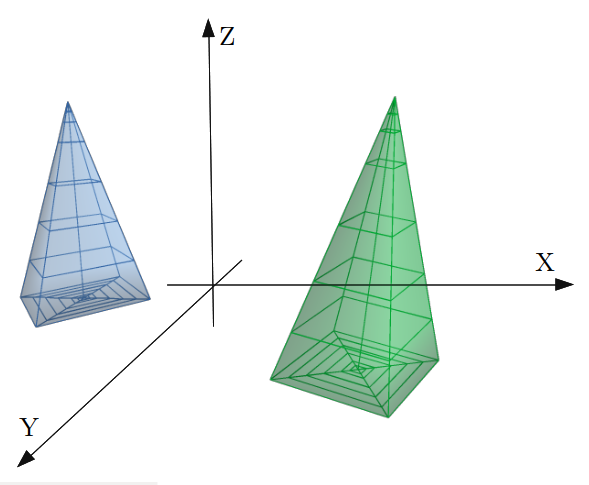
\includegraphics[width=0.8\linewidth, height=4.5cm]{Otros/PRE_1} 
			\caption{}
			%\label{fig:subim1}
		\end{subfigure}
		\begin{subfigure}{0.5\textwidth}
			\centering
			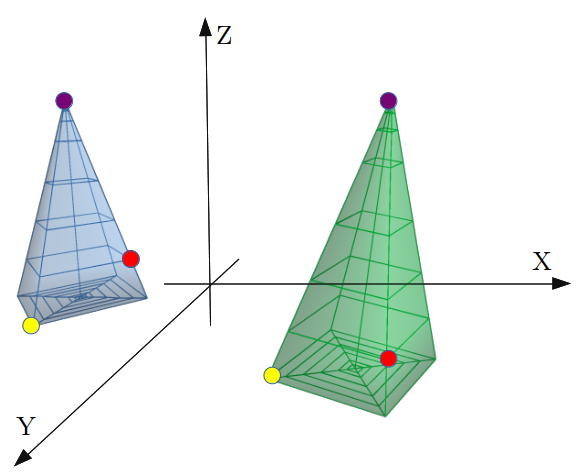
\includegraphics[width=0.8\linewidth, height=4.5cm]{Otros/PRE_2}
			\caption{}
			%\label{fig:subim2}
		\end{subfigure}	
		\caption{Selección de puntos en ambos conjuntos.}
		\label{fig:ex-pre}
\end{figure}
\item Llevar los primeros puntos seleccionados al origen de coordenadas.

\item Llevar los segundos a la parte positiva del eje $ X $ manteniendo fijos los anteriores.
\item Intentar aproximar lo máximo posible los otros puntos mediante una rotación alrededor del eje $ X $.
\end{enumerate}

\begin{figure}[h!]
	\begin{subfigure}{0.5\textwidth}
		\centering
		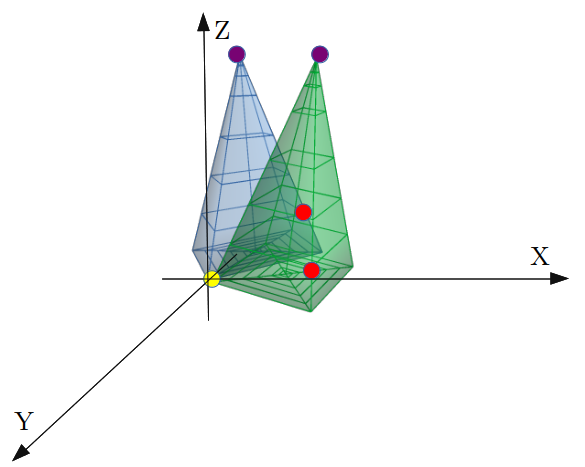
\includegraphics[width=0.8\linewidth, height=4.5cm]{Otros/PRE_3}
		\caption{Paso 2: llevar los primeros puntos al origen.}
	\end{subfigure}
	\begin{subfigure}{0.5\textwidth}
		\centering
		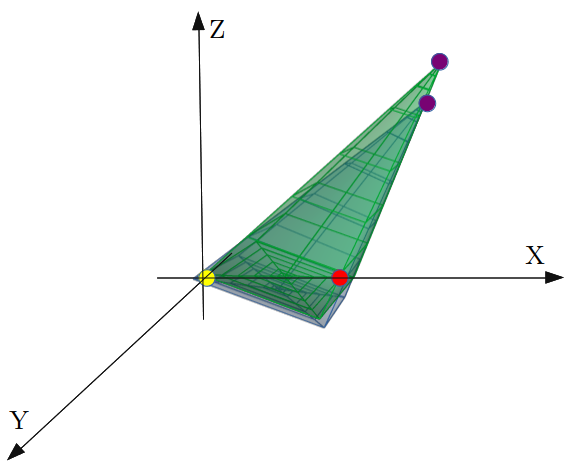
\includegraphics[width=0.8\linewidth, height=4.5cm]{Otros/PRE_4}
		\caption{Paso 3: llevar los segundos puntos al eje $ X $.}
	\end{subfigure}
	\begin{center}
		\begin{subfigure}{0.5\textwidth}
			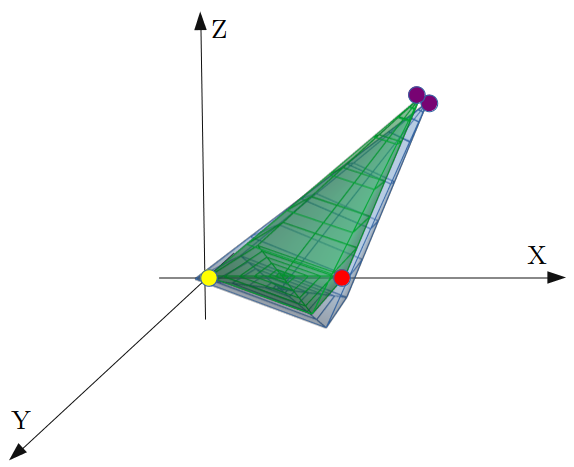
\includegraphics[width=0.8\linewidth, height=4.5cm]{Otros/PRE_5}
			\caption{Paso 4: aproximar lo máximo posible el punto restante.}
		\end{subfigure}
	\end{center}		
	\caption{Mecanismo de prealineado a partir de tres puntos.}
	\label{fig:ex-pre2}
\end{figure}


La figura \ref{fig:ex-pre2} muestra el proceso a seguir en estos últimos pasos. En secciones posteriores veremos un ejemplo práctico de este procedimiento.

\bigskip 
\begin{observacion}\label{ObsTmp}
El cálculo de los puntos más cercanos entre las nubes de puntos es un proceso muy costoso en tiempo.
\end{observacion}
Este paso del algoritmo es el que más tiempo ocupa de todo el proceso al tener una complejidad O($ N_p^2 $) en el peor de los casos. También tenemos que tener en cuenta el tamaño de los conjuntos de los puntos. La finalidad de este proceso es tener un modelo digital detallado y fiel a la realidad de un objeto real. Ello conlleva que las tomas se realicen con cierta calidad lo que hace que, incluso en modelos relativamente pequeños, cada una ronde los 2 millones de puntos. Si es un modelo más complejo podríamos llegar a los 20 millones. En estas situaciones, aplicar el método tradicional podría durar horas en completarse. \\

En esta situación, nos planteamos la posibilidad de una variante para no tener que comprobar todos y cada uno de los puntos en el proceso. En una primera aproximación, podríamos pensar en coger una subconjunto aleatorio de puntos de cada toma y aplicar el proceso descrito. Sin embargo, enseguida comprobamos que esta solución no es válida. Esto se debe a la convergencia local del método lo que nos conduce a las situaciones indeseadas que queremos evitar con el prealineado. Por ello, nos tenemos que plantear mecanismos más complejos que aseguren que se tienen en cuenta las tomas completas. \\

Un primer método sería usar usar índices espaciales como los \textit{octrees}. Los \textit{octrees} son estructuras jerárquicas que dividen el espacio en cubos denominados \textit{voxels}. Cada \textit{voxel} puede contener un máximo número de puntos por lo que si se supera dicho número el \textit{voxel} se dividiría en otros \textit{voxels} más pequeños. También podríamos imponer un profundidad máxima del árbol. En esta situación, solo deberíamos comprobar la distancia con un punto de cada \textit{voxel} y una vez se tiene, filtrar los puntos del modelo por esa distancia. \\

Otro mecanismo sería identificar alguna característica que nos permita clasificar los puntos. Como las tomas corresponden al mismo modelo, podemos suponer que la característica que buscamos se mantienen en cierta medida en ambos casos y solo tenemos que buscar el punto más cercano con aquellos que tienen características similares. Esta será la opción que nosotros usaremos para proponer alternativas basadas en este procedimiento y que veremos en la sección \ref{varNormal} .
\bigskip

\section{Ejemplos prácticos}\label{ejemPrac1}
En esta sección procedemos a probar el método implementado. Empezamos con un ejemplo parecido al artículo original. Los conjuntos de puntos para la prueba son:

\begin{table}[h!]
	\centering
	\begin{tabular}{| c | c | c |} 
		\hline
		$ x_1 $ & $ x_2 $ & $ x_3 $ \\
		\hline
		0.4389 & -0.0588 & 1.0699 \\ 
		0.4202 & 0.2052 & 1.1252 \\
		0.4201 &0.2539 & 1.1325 \\
		0.4495 & 0.0469 & 1.1260  \\
		0.4412 & 0.1796 & 1.1515 \\
		0.4826 & -0.0137 & 1.1359  \\
		0.4628 & 0.0703 & 1.1458 \\
		0.4700 & 0.1852 & 1.1765 \\
		\hline
	\end{tabular}
	\caption{Conjunto 1.}
	\label{table:1}
\end{table}

\begin{table}[h!]
	\centering
	\begin{tabular}{| c | c | c |} 
		\hline
		$ y_1 $ & $ y_2 $ & $ y_3 $ \\
		\hline
		0.7278 &0.0712 & 1.4610 \\ 
		0.7019 & 0.2480 & 1.4867 \\
		0.7621 & 0.1828 & 1.4720 \\
		0.7271 & 0.1769 & 1.4809  \\
		0.7067 & 0.0462 & 1.495 \\
		0.6438 & -0.0540& 1.4359  \\
		0.7247 & -0.0116 & 1.4385 \\
		0.6982 & 0.1981 & 1.4832 \\
		0.7700 & 0.2500 & 1.5000 \\
		0.8000 & -0.100 & 1.400 \\
		0.8300 & 0.3000 & 1.4500 \\
		\hline
	\end{tabular}
	\caption{Conjunto 2.}
	\label{table:2}
\end{table}

En la imagen \ref{fig:ICP_1} se muestran los puntos antes y después de aplicar una iteración de ICP. Notar que los del primer conjunto se han dibujado de color rojo y los del segundo de color verde. En esta ocasión no ha sido necesaria la etapa de prealineado al no haber una situación deseada tras la transformación. \\

\begin{figure}[h!]
	
	\begin{subfigure}{0.5\textwidth}
		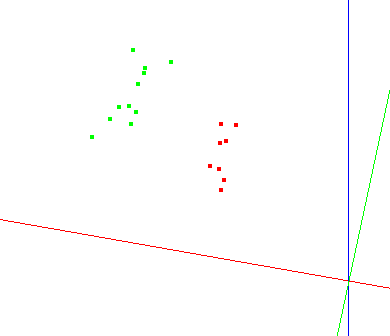
\includegraphics[width=0.7\linewidth, height=4cm]{ICP/prueba_ICP_1_1} 
		%\caption{Caption1}
		%\label{fig:subim1}
	\end{subfigure}
	\begin{subfigure}{0.5\textwidth}
		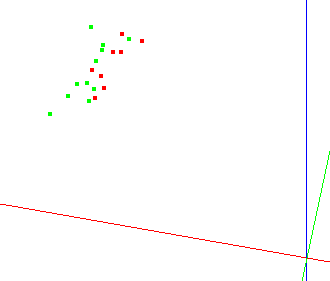
\includegraphics[width=0.7\linewidth, height=4cm]{ICP/prueba_ICP_1_2}
		%\caption{Caption 2}
		%\label{fig:subim2}
	\end{subfigure}
	
	\caption{Conjuntos de puntos antes y después de una iteración de ICP.}
	\label{fig:ICP_1}
\end{figure}

Según los datos calculados, la distancia media a pasado de $ 0.162697  $ a $ 0.00372463 $. El tiempo que ha tardado en realizar el proceso es de $ 0.00226548 $ segundos. La traslación y rotación expresada como cuaternio vienen dadas por 
\[
q_T =  (0.166271, 0.165485, 0.349303).
\]
\[
q_R = (0.0234481, 0.0238614, -0.154144, 0.987482).
\]

%%Besl y McKay también aportan en su artículo un estimación del la cantidad de operación necesarias en este caso. Para estos conjuntos con 8 y 11 puntos respectivamente ..... COMPRENDER. ¿Es necesario?. \\

El segundo ejemplo que vamos a probar consiste en un caso real, concretamente dos tomas de una escultura de un pie perteneciente a la Facultad de Bellas Artes de la Universidad de Granada tomadas con un escáner láser Faro Focus 130. Queremos alinear dos tomas obtenidas desde diferentes ángulos: \\

\begin{figure}[h!]
	
	\begin{minipage}[b]{0.5\textwidth}
		\centering
		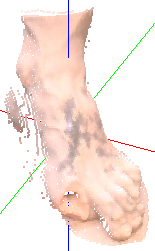
\includegraphics[width=0.5\textwidth]{ICP/prueba_ICP_2_1} 
		\caption*{Conjunto (1) con $ 7\,042 $ puntos.}
		%\label{fig:subim1}
	\end{minipage}
	\begin{minipage}[b]{0.5\textwidth}
		\centering
		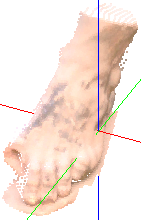
\includegraphics[width=0.5\textwidth]{ICP/prueba_ICP_2_2}
		\caption*{Conjunto (2) con $ 8\,334 $ puntos.}
		%\label{fig:subim2}
	\end{minipage}
	
	\caption{Tomas a alinear.}
	\label{fig:ICP_2}
\end{figure}

Tras la etapa de prealineado (los puntos seleccionados aparecen en la figura \ref{pre1}) se ha obtenido el resultado que muestran la figura \ref{pre2}. \\
\begin{figure}[h!]
	\begin{minipage}[b]{0.5\textwidth}
		\centering
		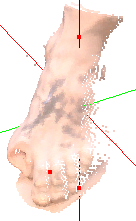
\includegraphics[width=0.5\textwidth]{ICP/prueba_ICP_2_3_1} 
		\caption*{Puntos clave del primer conjunto.}
		%\label{fig:subim1}
	\end{minipage}
	\begin{minipage}[b]{0.5\textwidth}
		\centering
		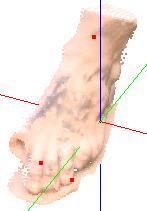
\includegraphics[width=0.5\textwidth]{ICP/prueba_ICP_2_3_2}
		\caption*{Puntos clave del segundo conjunto.}
		%\label{fig:subim2}
	\end{minipage}
	\caption{Etapa de prealineado.}
	\label{pre1}
\end{figure}
\begin{figure}[h!]
	
	\begin{minipage}[b]{0.5\textwidth}
		\centering
		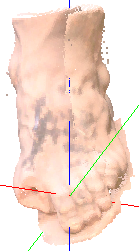
\includegraphics[width=0.5\textwidth]{ICP/prueba_ICP_2_3_3} 
		\caption*{Vista 1}
		%\label{fig:subim1}
	\end{minipage}
	\begin{minipage}[b]{0.5\textwidth}
		\centering
		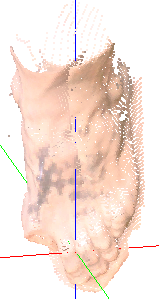
\includegraphics[width=0.5\textwidth]{ICP/prueba_ICP_2_3_4}
		\caption*{Vista 2}
		%\label{fig:subim2}
	\end{minipage}
	\caption{Vistas tras prealinear.}
		\label{pre2}
\end{figure}

A continuación, comenzamos usamos el algoritmo ICP. La tabla \ref{table:ICP2} recoge los datos tras cada iteración. Destacar que con distancia nos referimos a la distancia media entre los puntos y los más cercanos, es decir, lo que hemos notado como $ e_k $ y $ d_k $ en la sección \ref{algICP}. Por su parte, la figura \ref{fig:subim2}, muestra el resultado final tras las cinco iteraciones llevadas a cabo. \\

\begin{table}[h!]
	\centering
	\begin{tabular}{| c | c | c | c |} 
		\hline
		Iteración & Dist. antes ($ m^2 $)  & Dist. después ($ m^2 $) & Segundos \\
		\hline
		1 & 0.000449468 & 0.000328695 & 62.8672\\		 
		2 & 0.00027947 &  0.000251878 &  62.7888\\	
		3 & 0.000229901 & 0.000209142  & 62.8636\\
		4 & 0.000195308 &  0.000188837 & 63.059\\
		5 &  0.000186373 &  0.000185154 & 62.8259\\
		\hline
	\end{tabular}
	\caption{Resultados ajuste mediante ICP.}
	\label{table:ICP2}
\end{table}

\begin{figure}[h!]
	
	\begin{minipage}[b]{0.5\textwidth}
		\centering
		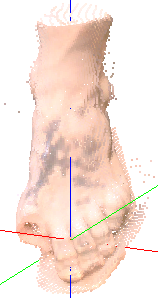
\includegraphics[width=0.5\textwidth]{ICP/prueba_ICP_2_3_5} 
		%\caption{Vista 1}
		%\label{fig:subim1}
	\end{minipage}
	\begin{minipage}[b]{0.5\textwidth}
		\centering
		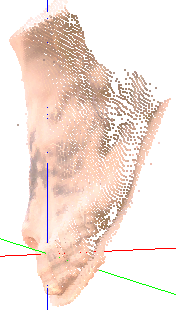
\includegraphics[width=0.5\textwidth]{ICP/prueba_ICP_2_3_6}
		%\caption{Vista 2}
	\end{minipage}
	\caption{Vistas tras cinco iteraciones del ICP.}
	\label{fig:subim2}
\end{figure}
En conclusión, vemos cómo el programa propuesto ha sido capaz de realizar un buen ajuste y por ello hemos conseguido un modelo más completo al original uniendo ambas tomas. Destacamos nuevamente la importancia que tiene en el proceso el prealineado. No solo na necesidad de hacerlo sino también la manera en la que sea lleva a cabo este proceso. Es posible que incluso incluyendo esta etapa el resultado no sea el deseado. Este comportamiento se debe como  ya hemos indicado a la convergencia local del método ICP. Las dos nubes de puntos tienen que estar los no solo lo suficientemente cerca sino también colocadas de tal manera que el algoritmo propuesto solo deba realizar un pequeño ajuste. \\

Por otro lado, también vemos que el tiempo empleado es elevado tal y como se indicó en la observación \ref{ObsTmp}: cada iteración ha durado algo más de un minuto. Hay que tener en cuenta que las nubes de puntos tomadas como modelo tienen un tamaño muy pequeño. En situaciones reales las tomas pueden tener millones de puntos lo que conllevaría mucho tiempo a la hora de aplicar el algoritmo e incluso sin la certeza de si el resultado es el que deseamos. En la siguiente sección planteamos unos métodos para acelerar este proceso.

%% \section{Aleatorios}